% Created 2023-04-23 Sun 22:05
% Intended LaTeX compiler: pdflatex
\documentclass[final, 12pt] {ubb_dolgozat}{book}
\usepackage[utf8]{inputenc}
\usepackage[T1]{fontenc}
\usepackage{graphicx}
\usepackage{longtable}
\usepackage{wrapfig}
\usepackage{rotating}
\usepackage[normalem]{ulem}
\usepackage{amsmath}
\usepackage{amssymb}
\usepackage{capt-of}
\usepackage{hyperref}
\usepackage{minted}
\submityear{2022}
\doctypeHU{Szakdolgozat}
\doctypeEN{Diploma Thesis}
\doctypeRO{Lucrare de licenta}
\specHU{Informatika}
\specEN{Computer Science}
\specRO{Informatică}
\titleHU{Felhasználói értékeléseken alapuló collaborative filtering algoritmusok kiértékelése funkcionális környezetben}
\titleEN{License thesis title}
\titleRO{Titlu lucrare licență}
\authorHU{Zediu Álmos-Ágoston}
\authorRO{Álmos-Ágoston Zediu}
\authorEN{Álmos-Ágoston Zediu}
\tutorHU{dr. Bodó Zalán}
\tutorRO{dr. Bodó Zalán}
\tutorEN{dr. Bodó Zalán}
\pagenumbering{gobble}
\author{Álmos-Ágoston Zediu}
\date{\today}
\title{Felhasználói értékeléseken alapuló collaborative filtering algoritmusok kiértékelése funkcionális környezetben}
\hypersetup{
 pdfauthor={Álmos-Ágoston Zediu},
 pdftitle={Felhasználói értékeléseken alapuló collaborative filtering algoritmusok kiértékelése funkcionális környezetben},
 pdfkeywords={},
 pdfsubject={},
 pdfcreator={Emacs 28.2 (Org mode 9.6.1)}, 
 pdflang={English}}
\usepackage{natbib}
\begin{document}

\maketitle
\tableofcontents


\chapter{Bevezetés}
\label{sec:org258b10f}
Napjainkban egyre nagyobb hangsúly kerül a különböző ajánló rendszerekre, algoritmusokra melyek felhasználási területe
igencsak kiterjedt, legyen akár szó e-commerce felületek termékajánlásáról, streaming szolgáltatások ízlésmeghatározásáról,
vagy pedig a közösségi média oldalak fő bevételforrásának számító személyes reklámajánlásáról.

A dolgozat fő tematikája három széles körben alkalmazott algoritmus, algoritmuscsalád ismertetése, előnyeinek és hátrányainak
bemutatása, körbejárva az implementációs nehézségeket, kiértékelési metrikákat és az adott algoritmusok megfelelő környezetben
való felhasználását.

A három bemutatott algoritmus a Slope One, mely egy lineáris regressziónál egyszerűbb ajánlási modell egyetlen
szabad paraméterrel, a Locality Sensitive Hashing, ami a hasonló ízléssel rendelkező felhasználók értékelési vektorait egy magas ütközési
rátával rendelkező hasítófüggvénnyel csoportosítja, és a Singular Value Decomposition mátrix faktorizációs módszer, ami a felhasználók
és az értékelt elemek közötti legfontosabb látens faktorokat hozza napvilágra.

Egy másik bemutatott szempont az algoritmusok Clojure nyelvben való implementálása.  A Clojure egy funkcionális Lispre alapuló nyelv, mely a JVM
platformon fut, nagy hangsúlyt fektet az adatvezérelt programozásra, az interaktív, REPL alapú fejlesztésre és a keretrendszerek helyett
az egyszerű könyvtárakra, melyeket az Unix filozófia alapján modulárisan használunk fel.

\chapter{{\bfseries\sffamily TODO} Az adathalmazról}
\label{sec:orge493ea2}
Az adathalmaz a Minnesotai Egyetem MovieLens adathalmaza, mely 100 000 értékelést tartalmaz 943 felhasználótól
1682 filmről. \citep{harperMovieLensDatasetsHistory2016}
\chapter{Clojure}
\label{sec:orgb838d60}
A Clojure egy dinamikus funkcionális nyelv, mely ötvözi a JVM platform előnyeit a Lisp nyelvek
kifejezőkészségével.
\section{Funkcionális nyelvekről kicsit általánosan.}
\label{sec:org1246615}
A funkcionális nyelvek fő alapelve az, hogy nincs mutálható memória, és ahelyett, hogy imperatív, egymáson
és programállapoton alapuló utasításokkal dolgozunk, előtérbe helyezzük a kifejezéseket, és a ``tiszta'' mellékhatásoktól
mentes függvényeket, melyeknek eredménye a bemeneti paraméterektől függ.

\section{Funkcionális programozás Clojureben}
\label{sec:orgf1d080a}
A Clojure fő filozófiája az egyszerű adatszerkezetekkel, főleg mapekkel való modellezése a problémáknak. Ahelyett, hogy
bonyolult absztrakciókat képezünk és enkapszuláljuk az adatainkat a rajtuk végzett műveletekkel (ezáltal ``objektumokat'',
és ``metódusokat képezve''), vagy pedig előbb bonyolult típusosztályokkal algebrai adatstruktúrákat képzünk, előtérbe
helyezzük az egyszerű adatstruktúrákat, és az egyszerű adatstruktúrákon operáló függvényeket.

A Clojureben a függvények az elsőrendű absztrakciók, képesek vagyunk akár argumentumként is kezelni őket, stb.

\begin{minted}[]{clojure}
(defn my-adder [a b] (+ a b))

(def my-five-adder (partial my-adder 5))

(map my-five-adder [1, 2, 3, 4])

\end{minted}

\begin{itemize}
\item \#'user/my-adder
\item \#'user/my-five-adder
\item (6 7 8 9)
\end{itemize}

\section{Perzisztens adatstruktúrák}
\label{sec:org1ee9e0e}
Egy lényegi kérdés ami felmerülhet funkcionális nyelvek esetén, az a memóriahasználat, és a futási idő problémája. Mivel minden változó alapvetően konstans, ezért minden egyes olyan
művelet, ami imperatív nyelvekben az eredeti adatstruktúra változtatását vette volna igénybe (új elem beszúrás, törlés, tulajdonság megváltoztatása), a funkcionális nyelvekben
egy ``módosított'' változatát adja vissza az eredeti algoritmusnak. Egy naiv háttérbeli implementáció esetén tehát egy esetleges tömb beszúrásnál le kellene másolni az egész tömböt.
Itt jön be a perziztencia, és a strukturális megosztás ötlete. Ha van olyan része a memóriának, ami változatlan marad az új adatstruktúrában is, fölösleges azon a memóriarészen levő
értékeket lemásolni, és több értelme van megosztani vele.

A Clojure alap adatstruktúrái az ideális hasítófákra vannak alapozva. \citep{jayasingheExtremeAmplitudeMassive2019} \citep{bagwellIdealHashTrees2001}. Egy konceptuális elképzelésért
rátekinthetünk erre a képre:

\begin{center}
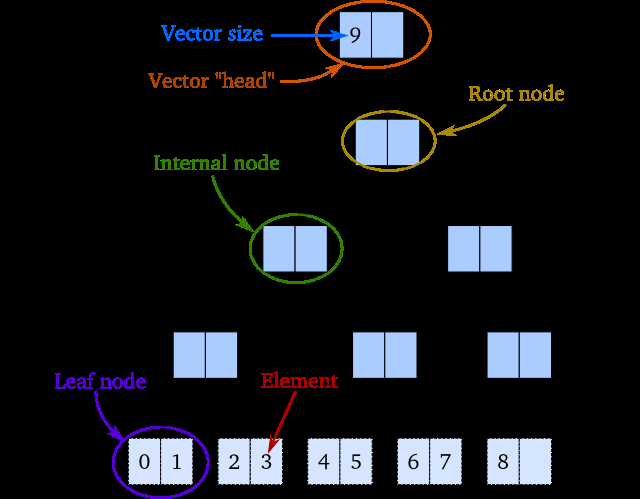
\includegraphics[width=.9\linewidth]{images/perzisztens-vektor.jpg}
\end{center}

A lényegi rész az, hogy ahhoz, hogy olyan adatstruktúrák, mint a vektorok performánsak legyenek, de perzisztensek, szükségünk van
specializált bináris fák felépítésére.

\section{Homoikonicitás}
\label{sec:orgac78198}
Ami talán leginkább megkülönbözteti a Lisp nyelvcsaládban levő nyelveket a többiektől, az a  homoikonicitás \citep{mcilroyMacroInstructionExtensions1960} tulajdonság, vagyis maga a programkód
formálható ugyanazzal a nyelvvel futás közben, mint amiben meg volt írva.

Hasonló viselkedést elérhetünk nem homoikonikus nyelvekben is, mint mondjuk a Java vagy a C\# reflection rendszere, vagy
pedig a Python dekorátor szintaxisa, viszont a Lisp nyelvek makrórendszereivel azért könnyebb valamilyen szinten dolgozni, mivel nincsenek speciálisan megkülönböztetve a programban
felhasznált adatstruktúrák szintaxisai, és a programot felépítő, elágazásokat, ismétlő ciklusokat, függvénydefiníciókat jelző nyelvi struktúrák szintaxisai.

Vegyük példának okáért a következő egyszerű programot:

\begin{minted}[]{clojure}
(defn add-list-numbers [number-list]
  (apply + number-list))

(add-list-numbers '(1 2 3 4 5))
\end{minted}

\begin{itemize}
\item \#'user/add-list-numbers
\item 15
\end{itemize}

Látható, hogy a függvénydefiníció kerek zárójelekbe írtuk, a függvény argumentumai pedig egy vektorszerű struktúrában kaptak helyet, utána pedig maga a függvényhívás is zárójelek között volt. Érdekes módon az átadott lista szintúgy zárójelezve adódott át, viszont raktunk elé egy aposztrófot is.

Erre azért volt szükség, mivel a Lisp nyelvekben a kerek zárójel listát jelöl, és minden lista, hacsak nem jelezzük aposztróffal, függvénymeghívással jár. Annak köszönhetően viszont, hogy ``listákban'' programozunk, képesek vagyunk a programrészleteinket mint lista, vektor, vagy halmazelemeket
módosítani átrendezni.

\subsection{Makrók}
\label{sec:org3a85caa}
A Lisp makrók olyan programszerkezetek, amelyek kódrészletet kapnak argumentumként, módosítják azt, és a módosított programrészlet eredményét futtatják végül le. Fontos megjegyezni, hogy a végső kód legenerálása fordítási időben történik, nem futási időben.

Egy jó példa arra, hogyan segíthet ez fejlesztésben és talán még fontosabb, adatelemzés során, az az úgynevezett ``threading'' makró.

\begin{minted}[]{clojure}
(defn generate-masked-grouped-ratings [dataset-path]
  (-> (load-ratings dataset-path)
      (tc/dataset)
      (tc/complete :user :item)
      (tc/group-by :user {:result-type :as-seq})))
\end{minted}

Szerepe tulajdonképpen abból áll, hogy az első logikai egységet ami a nyíl mellett áll, ``befűzi'' a következő függvényhívás
első argumentumaként és azon függvényhívás eredményét pedig ugyanúgy befűzi a következő függvényhívás első argumentumaként, és így tovább.

Bár talán komplikáltnak tűnhet egy hasonló funkcionalitás implementálása, ezen makró forráskódja mindössze 10 sor, és
kihasználja azt, hogy a ``formok'' (a Clojure kód kerek zárójelbe helyezett futtatható egysége) igazából listák, így a makró feladata egyszerűen a helyes futtatható lista megalkotása.

\begin{minted}[]{clojure}
(defmacro ->
  [x & forms]
  (loop [x x, forms forms]
    (if forms
      (let [form (first forms)
            threaded (if (seq? form)
                       (with-meta `(~(first form) ~x ~@(next form)) (meta form))
                       (list form x))]
        (recur threaded (next forms)))
      x)))
\end{minted}
\chapter{Algoritmusok}
\label{sec:org07732a4}
\section{Slope one}
\label{sec:orge5ab5e1}
A Slope One egy egyszerűen implementálható, de ennek ellenére meglepően jó eredményekkel
rendelkező algoritmuscsalád melyet Anna Maclachlan és Daniel Lemire jelentettek meg.
\citep{lemireSlopeOnePredictors2008}

Nevét onnan kapta, hogy a amíg az egyszerű lineáris regresszió esetén két paramétert becsülünk meg,
itt elég csak egy paraméter, leegyszerűsítve a \(f(x) = ax + b\) modellt egy \(f(x) = x + b\) modellre. Abban az esetben, mikor
felhasználói értékelésekről beszélünk nem egy adott termék vagy értékelendő tárgy individuális értékeléseit vizsgáljuk,
hanem az egy-egy tárgy értékelései közötti átlagos különbséget.

\begin{center}
\includegraphics[width=.9\linewidth]{images/slopeexample.png}
\end{center}


\subsection{Működési elv}
\label{sec:org79f1292}
Az algoritmus dióhéjban összesíti a tárgyak közötti szavazatkülönbségeket,
utána pedig ahhoz, hogy megközelítsük egy felhasználó ismeretlen szavazatát, összeadjuk a
létező szavazatait a vizsgálandó tárgy és az létező szavazatok közötti átlagos különbségekkel,
és súlyozott átlagot számolunk, ahol a súly az, hogy hányan szavaztak mindkét tárgyra.

Ha a felhasználó \(u\)-ként jelöljük, a szavazatai halmazát \(S(u)\)-ként, akkor egy \(j\) tárgyra
adott:

\begin{equation}
\hat{r}_{j|u} = \frac{\sum_{i \in S(u); i \not= j}{(\Delta{i,j} + u_{i})c_{j,i}}}{\sum_{i \in S(u) i \not= j} c_{j,i}}
\end{equation}

\citep{lemireSlopeOnePredictors2008}

Ahol \(c_{j,i} = card(S_{j,i}(R)\) vagyis a kardinalitása a \(j\) és \(i\)-re is szavazott embereknek.

\subsection{Implementáció}
\label{sec:org1b53c09}
Az ebben a szekcióban levő kód nagy része Henry Garner Clojureben való gépi tanulásról
szóló könyvéből lett átvéve, \citep{garnerClojureDataScience2015} , és a \textbf{top-n} ajánlási mechanizmussal együtt is alig tesz ki 50 sort.

Először a listakonstruktor elvű \textbf{for} makróval tárgy párokat generálunk, majd egy üres \textbf{map} asszociatív struktúrából kiindulva leredukáljuk ezeket a párokat egy mapre, melyben
minden az összes tárgyak közötti különbség el van mentve.

\begin{minted}[]{clojure}
(defn conj-item-difference [dict [i j]]
  (let [difference (-  (:rating j) (:rating i))]
    (update-in dict [(:item i) (:item j)] conj difference)))

(defn collect-item-differences [dict items]
  (reduce conj-item-difference dict
          (for [i items
                j items
                :when (not= i j)]
            [i j])))

(defn item-differences [user-ratings]
  (reduce collect-item-differences {} user-ratings))
\end{minted}

Ezután elmentjük a különbségek átlagát, és a közös szavazók számát.

\begin{minted}[]{clojure}
(defn summarize-item-differences [related-items]
  (let [f (fn [differences]
            {:mean  (s/mean differences)
             :count (count  differences)})]
    (map-vals f related-items)))

(defn slope-one-recommender [ratings]
  (->> (item-differences ratings)
       (map-vals summarize-item-differences)))
\end{minted}

A felhasználási lépésben, amikor egy adott tárgyra szeretnénk értékelést megsaccolni,
hozzáadjuk a meglevő szavazatokat a különbségekhez és elvégezzük a súlyozott átlagolást.

\begin{minted}[]{clojure}
(defn candidates [recommender {:keys [rating item]}]
  (->> (get recommender item)
       (map (fn [[id {:keys [mean count]}]]
              {:item id
               :rating (+ rating mean)
               :count count}))))

(defn weighted-rating [[id candidates]]
  (let [ratings-count (reduce + (map :count candidates))
        sum-rating (map #(* (:rating %) (:count %)) candidates)
        weighted-rating (/ (reduce + sum-rating) ratings-count)]
    {:item id
     :rating weighted-rating
     :count  ratings-count}))
\end{minted}

A top-n ajánlás már csak annyit ad hozzá, hogy elvégzi az egész adathalmazra a
megközelítéseket, kiveszi a vizsgált felhasználó már értékelt tárgyait, és csökkenő sorrendbe helyezi az értékeléseket.

\begin{minted}[]{clojure}
(defn slope-one-recommend [recommender rated top-n]
  (let [already-rated  (set (map :item rated))
        already-rated? (fn [{:keys [id]}]
                         (contains? already-rated id))
        recommendations (->> (mapcat #(candidates recommender %)
                                     rated)
                             (group-by :item)
                             (map weighted-rating)
                             (remove already-rated?)
                             (sort-by :rating >))]
    (take top-n recommendations)))
\end{minted}

\section{Locality sensitive hashing}
\label{sec:org2a7ee75}
A Locality Sensitive Hashing egy olyan hasítófüggvényekre alapuló módszer, ami a legtöbb hasítófüggvény implementációval ellentétben nem minimizálja az ugyanolyan kimenetek, kulcsok
számát, hanem maximalizálja, mivel a hasonló tárgyak, (esetünkben szavazatvektorok) hasonló kimenettel kell rendelkezzenek.

\subsection{Definíció}
\label{sec:orgd435de7}
Egy LSH séma egy olyan \(F\) hasítófüggvénycsalád, melyekre igaz, hogy a valószínűsége annak,
hogy két \(x\), \(y\) objektum függvényértéke megegyezik, megegyezik a két függvény hasonlósági távolságával valamilyen metrika szerint. \citep{charikarSimilarityEstimationTechniques}

\begin{equation}
Pr_{h \in F} [h(x) = h(y)] = sim(x, y)
\end{equation}

ahol \(sim(x,y) \in [0,1]\) természetesen.

Ezzel egyrészt csoportosítani tudjuk a potenciálisan hasonló ízléssel rendelkezőeket, és ugyanakkor kompaktan, kevés helyfelhasználással később is fel tudjuk használni ezen csoportokat, ami segít a futási időn is persze.

\subsection{Véletlenszerű hiperterekre alapuló LSH}
\label{sec:orged3279e}
Az ötlet a következő: egy \(R^{d}\)-ből levő vektorcsoport esetén mintavételezzünk egy normál eloszlású \(\overrightarrow{r}\) \(d\) dimenziós vektort. Ennek a vektornak a függvényében definiálhatjuk a következő \(h_{\overrightarrow(r)}\) függvényt:

\begin{equation}
h_{\overrightarrow(r)} (\overrightarrow{u})= \begin{cases}
                                                1 & ha \overrightarrow{r} * \overrightarrow{u} \ge 0 \\
                                                0 & ha \overrightarrow{r} * \overrightarrow{u} < 0
                                                \end{cases}
\end{equation}


Ekkor \(\overrightarrow{u}\) és \(\overrightarrow{v}\) esetén igaz lesz, hogy:


\begin{equation}
Pr_{h \in F} [h(x) = h(y)] = 1 - \frac{\theta(\overrightarrow{ u }, \overrightarrow{ v })}{\pi}
\end{equation}
\citep{charikarSimilarityEstimationTechniques}

Vagyis annak a valószínűsége, hogy két vektor egyenkénti skaláris szorzata a véletlenszerűvel és az erre alkalmazott előjel függvény kimenete ugyanaz legyen megegyezik a két vektor között
bezárt szög koszinuszával.
Ezt először Goemans és Willamson bizonyította \citep{goemansImprovedApproximationAlgorithms1995} egy a MAX-CUT relaxációjával foglalkozó cikkükben.

Intuitívan arról van szó, hogy ha veszünk egy \(d\)  dimenziós hiperteret, ahol \(d\) az adathalmazunkban levő tárgyak száma, akkor minden felhasználót el tudunk helyezni ebben a
hipertérben, hisz a szavazataik meghatározzák a pozíciójukat, hisz d dimenziós vektorok.

Egy véletlenszerűen felvett vektor normálvektora egy a hiperteret kettéosztó hipersíknak, vagyis
a vele való skaláris szorzat előjele meghatározza, hogy egy pont a hipersík melyik felén helyezkedik el.

Elég ilyen hipersíkot felvéve ki tudunk alakítani csoportokat, akik több hipersíknak is ugyanazon
a felén vannak, ebből következve hasonlóak.


\begin{center}
\includegraphics[width=.9\linewidth]{images/randomprojection.png}
\end{center}
\citep{RandomProjectionLocality}

\subsection{{\bfseries\sffamily TODO} Implementáció}
\label{sec:orgdcc24b6}
Az első lépés a random normálvektorok legenerálása:

\begin{minted}[]{clojure}
(defn generate-random-vectors [d nbits]
  (nrand/rand-normal! 0 1 (nnat/dge d nbits)))
\end{minted}

A függvény amely kiszámítja mely ``vödörbe kerül'' egy felhasználó az értékelési vektora alapján

\begin{minted}[]{clojure}
(def threshold
  "The sign function which translates a value into a binary 1 or 0."
  (fn [x]
    (if (> x 0.0)
      1.0
      0.0)))

(defn calculate-lsh-hash
  "Used to calculate the LSH hash of a random vector."
  [user-vector rand-normals]
  (. Integer parseInt (->> (ncore/mv rand-normals user-vector)
                           (fmap threshold)
                           (into [])
                           (map int)
                           (apply str)) 2))

\end{minted}

A függvény amely elvégzi a ``vödör'' generálást, és feltölti őket.

\begin{minted}[]{clojure}
(defn generate-lsh-buckets
  "Generating the buckets for the stuff."
  [all-items grouped-ratings rand-normals]
  (loop [current-rating (first grouped-ratings)
         remaining-ratings (rest grouped-ratings)
         current-user (get-in current-rating [:user 0])
         buckets {}]
    (let [sparse-vector (-> (get-sparse-ratings all-items current-rating)
                            (get-sparse-vector))
          lsh-hash (calculate-lsh-hash sparse-vector rand-normals)
          new-buckets (if (contains? buckets lsh-hash)
                        (update buckets lsh-hash conj current-user)
                        (conj buckets [lsh-hash [current-user]]))]
      (if (empty? remaining-ratings)
        new-buckets
        (recur (first remaining-ratings) (rest remaining-ratings) (get-in (first remaining-ratings) [:user 0]) new-buckets)))))
\end{minted}

\section{Singular Value Decomposition (SVD)}
\label{sec:org65ba81c}
\subsection{Definíció}
\label{sec:org408bf58}
A Singular Value Decomposition (röviden SVD) egy mátrix faktorizációs módszer, melyben egy \(m  \times  n\) mátrixot felbontunk
\(M=U \Sigma V^{*}\) módon, ahol \(U\) egy \(m \times n\) alakú unitáris mátrix, \(\Sigma\) egy \(m \times n\) alakú diagonális mátrix, \(V\) pedig egy \(n \times n\)
unitáris mátrix. \(\Sigma\) átlón elhelyezkedő értékei a négyzetgyökei \(M * M\) sajátértékeinek, és sok SVD implementációban az értékek
csökkenő sorrendben jelennek meg \(\Sigma\) főátlóján.

\subsection{Felhasználás ajánlórendszerekben}
\label{sec:orge4fc295}
Hasznossága abban rejlik, hogy ha kiválasztjuk az \(r\) legnagyobb singular value-t (vagy röviden s-értéket) akkor meg tudjuk közelíteni az eredeti \(M\) mátrixot, egy másik, \(\widetilde{M}\) mátrixxal, ahol
\(rank(\widetilde{M}) = r\) \citep{eckartApproximationOneMatrix1936a}. Ez azért tud hasznos lenni ajánlórendszerekben, mivel ezáltal le tudjuk redukálni az eltárolandó felhasználó-értékelt objektum
kapcsolatok számát, és csak a redukált \(r\) rangú \(M, \Sigma, V^{*}\) mátrixokat tárolva helyet spórolunk, ugyanakkor ki tudjuk emelni az \(r\) legfontosabb ``látens faktort'', amik megadják az összefüggést
bizonyos felhasználók és bizonyos filmekre adott értékelések között.

\subsection{Implementáció}
\label{sec:orgdd31aa7}
Az alkalmazott implementáció alapjául Badrul N. Sarwar, George Karypis etc, Minnesotai Egyetem kutatóinak cikke szolgál, \citep{sarwarApplicationDimensionalityReduction2000}
és felbontható a következő stádiumokra:

Az implementációban a normalizálás az objektumok átlagos pontszámai alapján történtek, vagyis csoportosítva lettek a szavazatok objektum szerint és onnan kivontuk az átlagszavazatot:

\begin{minted}[]{clojure}

(def multiple-averages (-> grouped-ratings
                    (tc/complete :user :item)
                    (tc/group-by :item {:result-type :as-seq})))

(def averages
(map
    (fn [group]
    (let [mean (-> (tc/aggregate group #(dfn/mean (% :rating)))
                    (tc/get-entry "summary" 0))
            normalized-group (-> (tc/replace-missing group :rating :value mean)
                                (tc/update-columns :rating [(partial map #(- % mean))]))]
        {:normal normalized-group
        :mean mean})) multiple-averages))
\end{minted}

Az átlagos értékelések el lettek mentve, hogy az adathalmaz rekonstrukciójakor de-normalizálni tudjuk a szavazatokat, megkapva az előrejelzett értékeléseket.

Az SVD kiszámítása a LAPACK lineáris algebra könyvtár Intel MKL implentációja alapján történik.

\begin{minted}[]{clojure}

(def svd (-> (nnat/dge 1680 943 (:rating new-normal))
            (nlin/svd true true)))

\end{minted}

Az adathalmaz rekonstrukciója során kiválasztjuk a 14 legnagyobb s-értéket, ugyanakkor az \(U\) és \(V^{*}\) mátrixok almátrixait, gyököt vonunk a
redukált \(\Sigma\) mátrixokból, és újra összeszorozzuk őket, megkapva a 14-es ranggal rendelkező \(\widetilde{M}\) mátrixot.

\begin{minted}[]{clojure}

(def sigma (-> (:sigma svd)
                (ncore/submatrix 14 14)))
(def u (ncore/submatrix (:u svd) 1680 14))
(def vt (ncore/submatrix (:vt svd) 14 943))
(def s_root (nvmath/sqrt sigma))
(def usk (ncore/mm u s_root))
(def skV (ncore/mm s_root vt))
(def usv (ncore/mm usk skV))

\end{minted}

\bibliographystyle{./abbrvnat_hu.bst}
\bibliography{/home/hrothgar32/Documents/allamvizsga/allamvizsga}
\end{document}